\documentclass[12pt]{article}

\pagestyle{empty}
%\setlength{\topmargin}{0in}
%\setlength{\headheight}{0in}
%\setlength{\headsep}{0in}
\usepackage[hmargin=2cm,vmargin=2cm]{geometry}


\usepackage{amssymb}
\usepackage{latexsym}
\usepackage{amsmath,amsthm}
\usepackage{enumerate}
\usepackage{multicol}
\usepackage{hyperref}
\usepackage{fancyhdr}
\usepackage{graphicx}
\usepackage{ragged2e}

\pagenumbering{gobble}

%\pagestyle{fancy}
%\chead{\Large Partial Fraction Decomposition}
%\lfoot{\footnotesize{Adapted from \textit{Thomas' Calculus:Early Transcendentals}}}
\cfoot{\hspace{.5cm}\thepage}
%\rfoot{\copyright Tracy Weyand}
\renewcommand{\headrulewidth}{0pt}
\renewcommand{\footrulewidth}{1pt}

\setlength\parindent{0pt}
\begin{document}

\begin{center}
\scalebox{3}{Belphegor's Prime}

\vfill

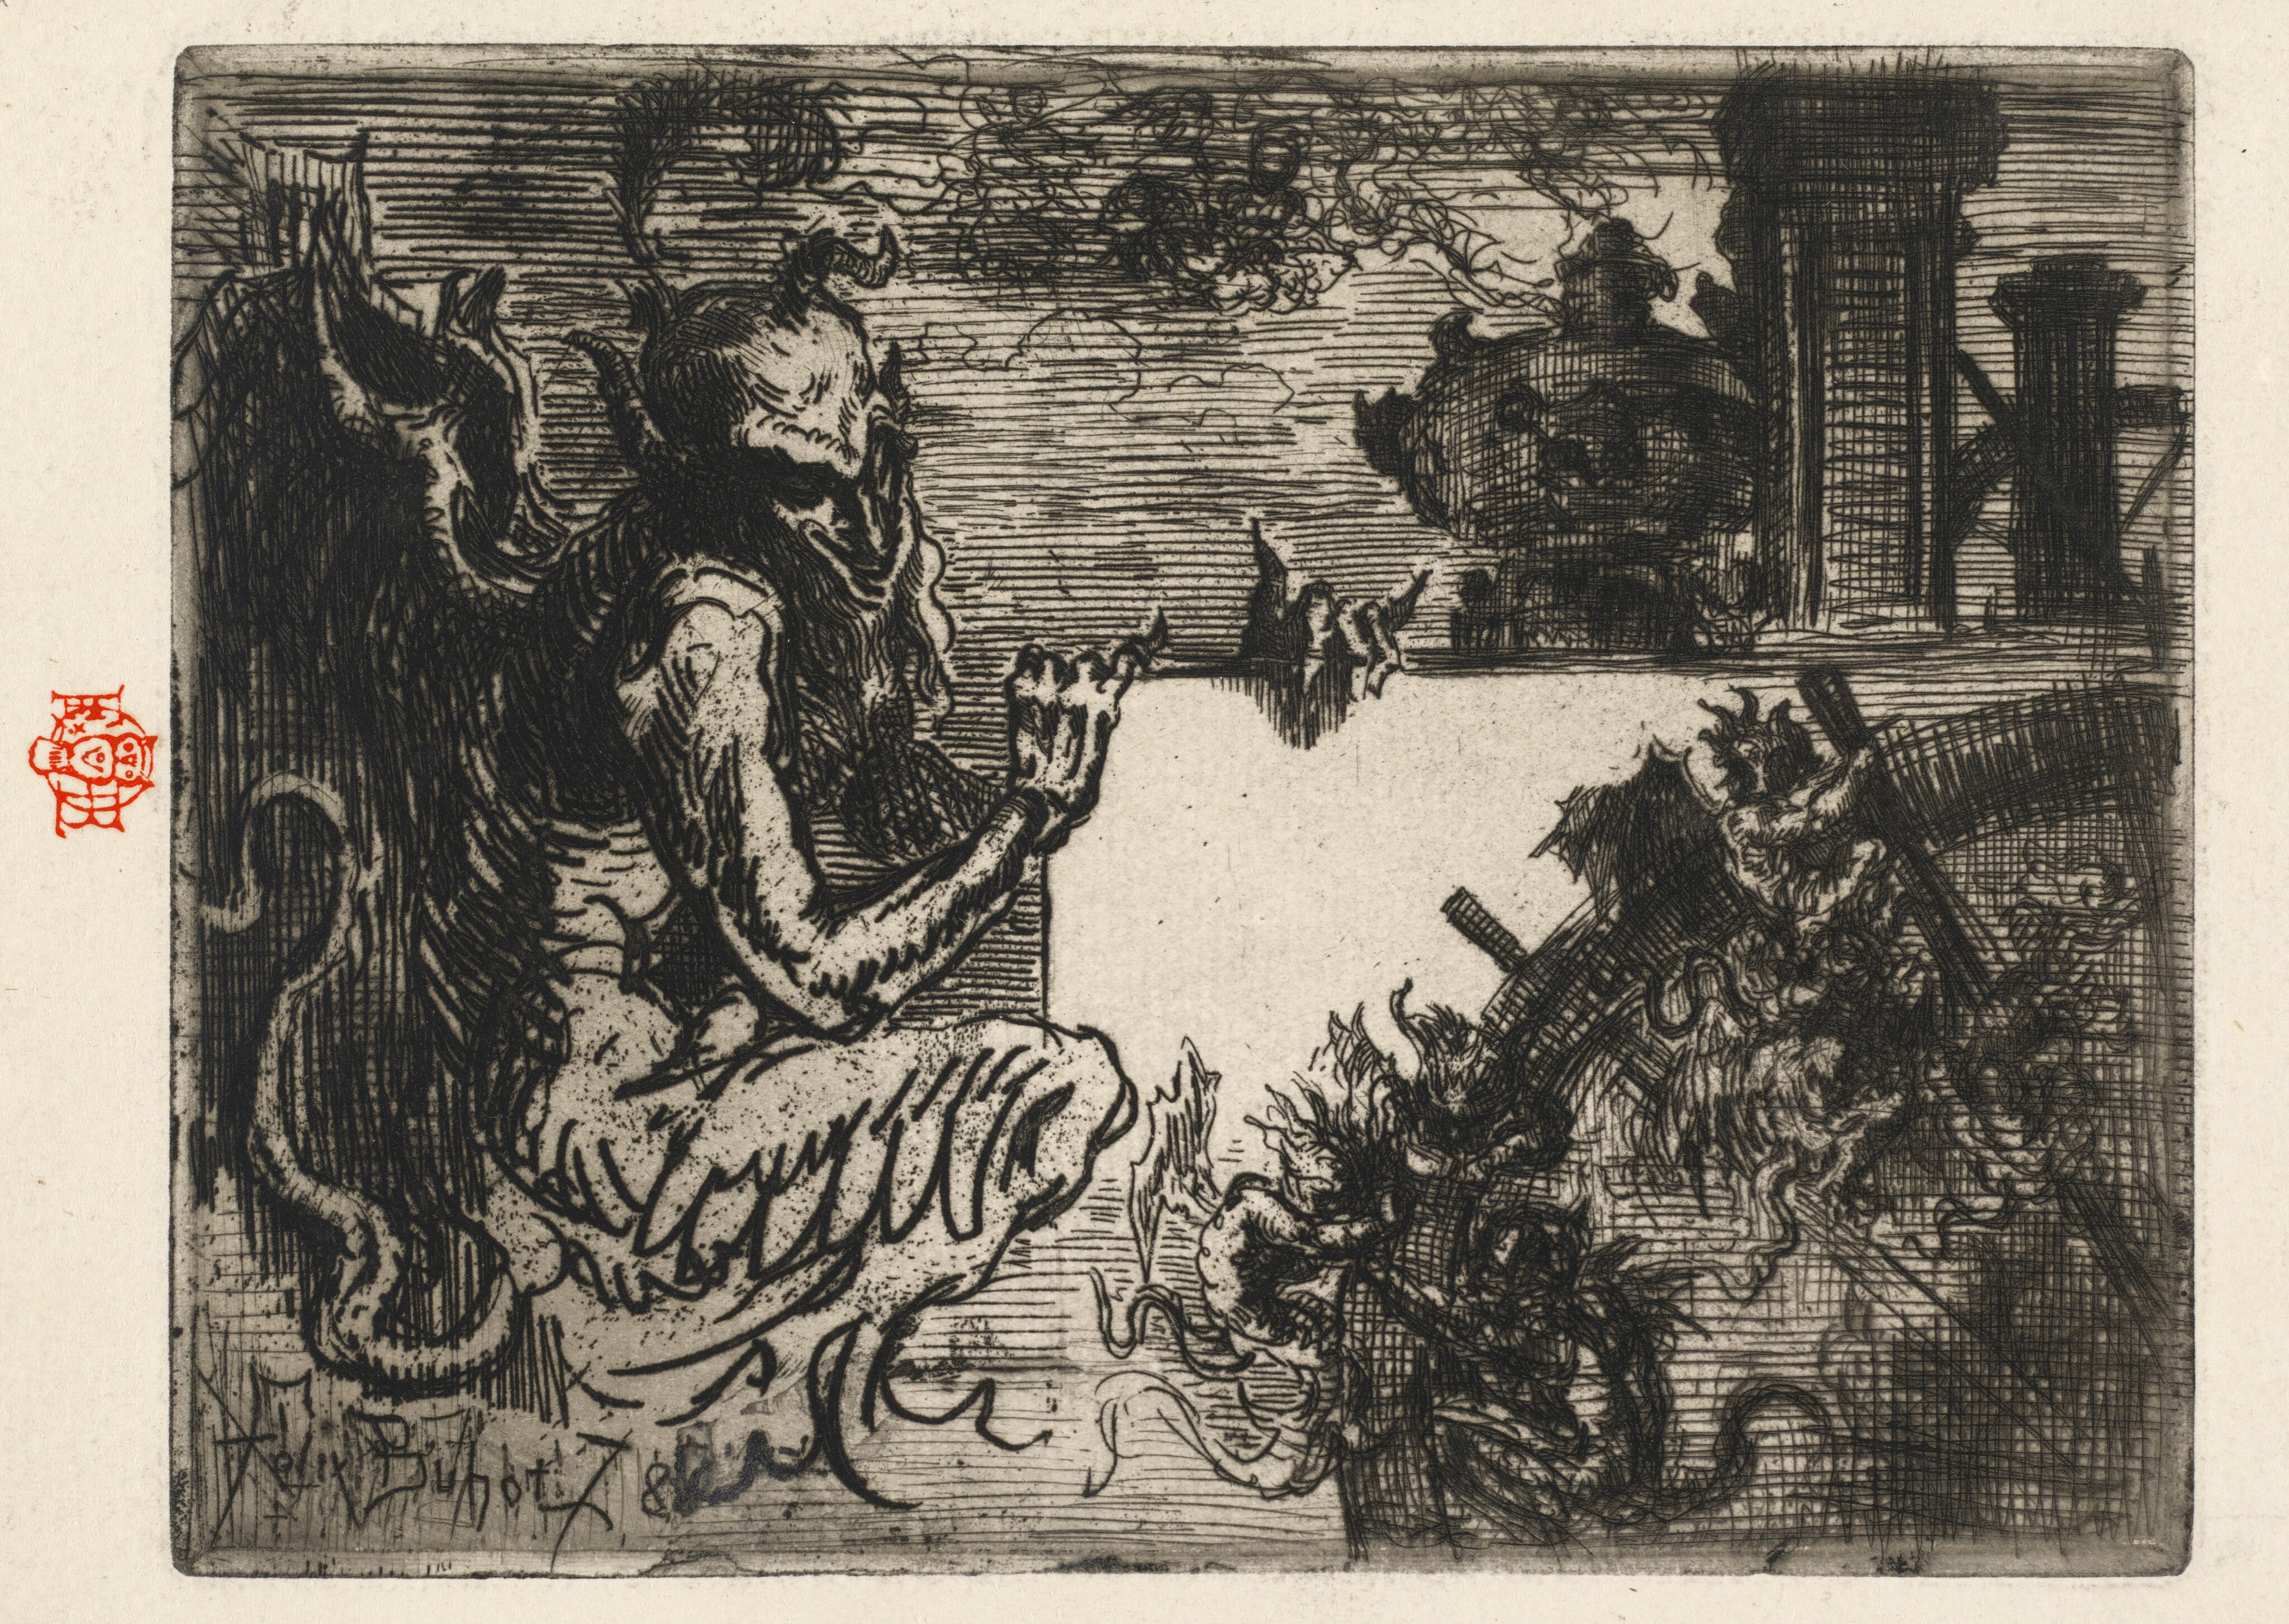
\includegraphics[scale=0.1]{img/the_demon_printer_2008.1.1}

The Demon Printer, Félix-Hilaire Buhot, 1878
\end{center}

\vfill

$$
\scalebox{2}{\rotatebox[origin=c]{180}{$\pi$} = 1000000000000066600000000000001}
$$

\vfill

\justifying
{{\large The Belphegor numbers are a sequence of integers which go $16661$, $1066601$, $100666001$, and so on.
Each Belphegor number is a palindrome; they are the same forwards and backwards.
Each contains the number $666$, which is associated with the devil in Western culture.}

\vfill

{\large Some of the Belphegor numbers are prime numbers, meaning that their only divisors are one and themselves.
The first Belphegor number that is prime is $16661$.
The next prime in the sequence is the number $\rotatebox[origin=c]{180}{$\pi$}$ shown above.
There are thirteen zeroes on either side of $666$, for a total of thirty-one digits.
Thirteen is considered to be unlucky in Western culture.
Not only that, thirteen (13) written backwards is thirty-one (31)!}

\vfill

{\large If we continue to add zeroes to the Belphegor numbers, there are more Belphegor primes.
The next Belphegor prime is a $1$ followed by $42$ zeroes, then $666$, then another $42$ zeroes and finally another $1$. The Belphegor prime after that has $506$ zeroes on either side of the $666$. What comes next?}}


\vfill

\noindent \textbf{The Demon Printer, 1878} https://www.nga.gov/collection/art-object-page.139842.html\\
\textbf{Belphegor's prime} https://en.wikipedia.org/wiki/Belphegor\%27s\_prime\\
\textbf{Indices of Belphegor primes} https://oeis.org/A232448


\end{document} 